\section{Empirical Results}
\label{sec:results}

We evaluate oracle erosion across $N = \BenchEligible$ flaky tests in $\BenchProjects$ repositories and 1,243 unique held-out candidate patches. We first quantify erosion prevalence and developer pull-request boundaries (RQ1), then diagnose why static guards miss behavioral shifts (RQ2) before assessing fail-closed mutation gating, asymmetric CI cost, and runtime overhead (RQ3--RQ4).

\subsection{RQ1: Prevalence of Silent Oracle Erosion and Pull-Request Boundaries}
\label{sec:rq1}

\paragraph{Historical Repair Artifacts.}
Silent oracle erosion is already pervasive in published flaky-test repair artifacts (Table~\ref{tab:b1_sota}). Among official upstream passing entries from \textsc{FlakyDoctor} GPT-4, nearly half compile verbatim and pass stability reruns, yet \BOneGptLeakPct{} of those stabilized patches silently drop baseline fault obligations. That erosion lowers operational sound-fix yield by 12 percentage points. By contrast, none of the four matched and stabilized \textsc{FlakyDoctor} Magicoder patches erode obligations, though four patches are too few to support model-level conclusions.

Python suite-search patching exhibits nearly the same erosion rate as LLM-based Java repair. Among partner-matched official \textsc{iPFlakies} entries, \BOneIpfLeakPct{} of stabilized fixes lose baseline obligations, opening a 13-point gap between apparent stabilization and sound repair. Silent erosion is therefore not unique to language models. Whenever a repair pipeline rewards green execution without checking fault detection, both search-based splicers and generative agents gravitate toward edits that silence intermittent failures at the cost of weaker assertions or shallower fixture states.

\begin{table}[t]
\centering
\footnotesize
\setlength{\tabcolsep}{3.0pt}
\caption{Audit of official upstream passing patches from \textsc{FlakyDoctor} and partner-matched \textsc{iPFlakies} artifacts under unified attribution. Bold marks silent oracle erosion among $W^+$-passing fixes.}
\label{tab:b1_sota}
\begin{tabular}{lrrrrrrr}
\toprule
Historical Artifact Cohort & Avail. & Mism. & Comp. & Pass@$W^+$ & Eroded & Leak ($W^+$) & SoundFix \\
\midrule
FlakyDoctor GPT-4 (official pass) & 75 & 20 & 38 & 33 (44.00\%) & \textbf{9} & \textbf{27.27\%} & 24 (32.00\%) \\
FlakyDoctor Magicoder (official pass) & 13 & 6 & 4 & 4 (30.77\%) & \textbf{0} & \textbf{0.00\%} & 4 (30.77\%) \\
iPFlakies (partner-matched) & 77 & 0 & 60 & 42 (54.55\%) & \textbf{10} & \textbf{23.81\%} & 32 (41.56\%) \\
\bottomrule
\end{tabular}
\end{table}


\paragraph{Modern LLM Backbones Across Five Models.}
Unconstrained LLM repair loops show consistent erosion rates across all five models from four vendors (Figure~\ref{fig:inflation_gap}, Table~\ref{tab:k5_operational}, and Table~\ref{tab:crossfamily_r1}). Under multi-round validation, API reasoning-token limits truncated one eligible test on DeepSeek Flash and 15 on DeepSeek V4 Pro, whereas confirmatory Qwen 3.7 Plus completed the full cohort. Silent erosion affects roughly one-fifth to one-quarter of stabilized patches on every backbone. Combined with the explicit \emph{Unver.} column in Table~\ref{tab:k5_operational}---unverified shared-scope partner edits plus one indeterminate target timeout on DeepSeek Flash and DeepSeek V4 Pro Unconstrained---these losses open a Proxy Inflation Gap of 24 to 26 percentage points across backbones.

Single-pass screening across two additional model families confirms that this gap generalizes beyond DeepSeek and Qwen. Without multi-round retries, unconstrained Kimi K2.5 leaks 26.8\% eroded patches among its stabilized outputs, and GLM-5 leaks 25.6\%. Across both reasoning and non-reasoning models, green stability checks overstate sound repair rates by roughly a quarter. This uniformity points to a structural incentive flaw rather than a quirk of any single model family. Because stabilization checks penalize every flaky failure immediately but never penalize a missing assertion check, stronger models simply become more adept at finding permissive edits that turn tests green quickly.

\begin{figure*}[t]
\centering
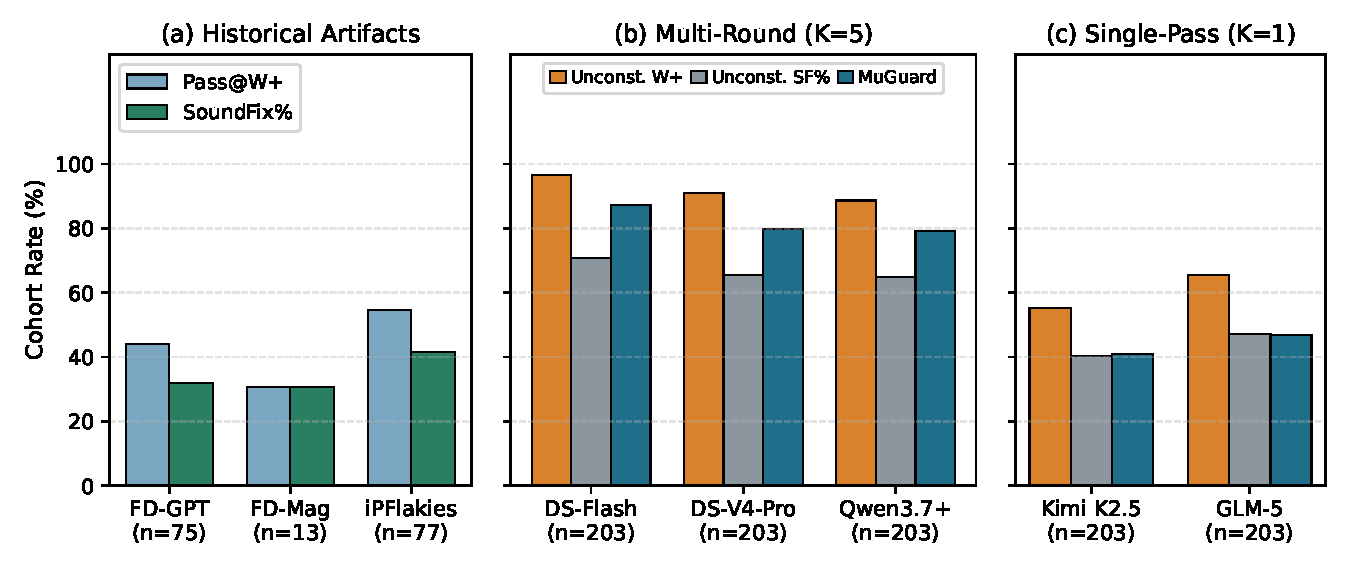
\includegraphics[width=0.98\textwidth]{figures/fig1_inflation_gap_models.pdf}
\caption{Apparent stabilization pass rate versus operational sound-fix rate across historical artifacts, multi-round LLM repair, and single-pass cross-family screening.}
\label{fig:inflation_gap}
\end{figure*}

\paragraph{Developer Pull Requests and the False-Rejection Boundary.}
Auditing real human fixes exposes both the false-rejection cost and the incomplete recall of strict mutation gating (Table~\ref{tab:pr_adjudication}). Across $\PRTotalInstances$ Java instances from $\PRDistinctURLs$ GitHub pull requests, 45 test-only fixes apply cleanly and 43 pass stability reruns, including all 24 order-dependent cases. Focusing on the 16 merged fixes that stabilize, Syntactic Guard rejects one, Structural Guard rejects three, and \textsc{MuGuard-Flake} rejects two. Diff adjudication---corroborated at 93.0\% agreement ($\kappa = 0.63$) by our blinded cross-audit---reveals opposite semantics for those two rejections: one Fastjson pull request legitimately enables deterministic map-key sorting, and a Nacos pull request replaces exact JSON equality with partial substring checks that genuinely weaken the oracle.

Across all $\PRLegitTotal$ verified legitimate test-only repairs, strict \textsc{MuGuard-Flake} gating rejects eight fixes, a \PRLegitFalseRejMuGuardPct{} false-rejection rate (or 22.5\% if the single Apache Avro responsibility-shift fix is included). Those eight false rejections stem from two concrete patterns: three Fastjson canonicalization fixes that bypass unsorted serialization branches, and five Visualee fixtures whose \texttt{@Before} singleton cleanup lowers PIT kill counts without altering any assertion. Conversely, manual review surfaced three genuine weakening pull requests among stabilized fixes. \textsc{MuGuard-Flake} and Structural Guard both catch the Nacos substring downgrade, and two subtle merged weakenings in Commons Collections and Apollo retain all default PIT kills and escape every gate.

These pull-request cases sharpen how strict mutation gating should be interpreted in practice. A strict gate does not separate legitimate fixes from broken ones with perfect precision, because valid canonicalization or fixture cleanup can legitimately change which production branches a test traverses. At the same time, default bytecode operators cannot expose every subtle relational weakening, such as dropping a cross-entry key-to-value bijection. Strict mutation gating therefore operates as an auditable safety filter with concrete false-rejection and false-negative boundaries rather than an omniscient oracle.

\begin{table}[t]
\centering
\scriptsize
\setlength{\tabcolsep}{2.4pt}
\caption{Gate rejection and weakening-detection rates across $W^+$-passing test-only developer pull requests comparing static, coverage, cross-vendor LLM-judge, strict \textsc{MuGuard-Flake}, and witness-augmented hybrid triage.}
\label{tab:pr_adjudication}
\begin{tabular}{llrrrrr}
\toprule
PR Cohort & $n$ & Structural & Coverage$^{\dagger}$ & LLM-Judge & MuGuard & MuGuard+Triage \\
\midrule
Merged Test-Only ($W^+$) & 16 & 3/16 (18.75\%) & 1/13 (7.7\%) & 2/16 (12.5\%) & 2/16 (12.50\%) & \textbf{1/16 (6.3\%)} \\
Legitimate Fixes (Primary) & 39 & 4/39 (10.3\%) & 2/32 (6.3\%) & 3/39 (7.7\%) & 8/39 (20.5\%) & \textbf{0/39 (0.0\%)} \\
Legit.\ + Shift (Sens.) & 40 & 4/40 (10.0\%) & 2/32 (6.3\%) & 3/40 (7.5\%) & 9/40 (22.5\%) & \textbf{0/40 (0.0\%)} \\
\midrule
Genuine Weakening (TP) & 3 & 1/3 (33.3\%) & 0/2 (0.0\%) & \textbf{3/3 (100\%)} & 1/3 (33.3\%) & 1/3 (33.3\%) \\
\bottomrule
\end{tabular}
\par\smallskip\parbox{0.97\textwidth}{\scriptsize\textit{Note:} Syntactic Guard rejects 1/39 (2.6\%) legitimate PRs and catches 0/3 weakenings. $^{\dagger}$JaCoCo executed on 34/43 Java PRs (9 blocked by upstream Maven \texttt{argLine} conflicts). LLM-Judge uses cross-vendor Qwen 3.7 Plus (Zhipu GLM-5 yields 2/39 = 5.1\% false rejections and 3/3 weakenings). Under our stricter 10-session blinded Codex ensemble rubric (Fleiss' $\kappa=1.00$), which classifies Visualee global singleton wipes as responsibility shifts, strict \textsc{MuGuard-Flake} rejects only 1/29 (3.4\%) strictly contract-preserving PRs.}
\end{table}


\medskip
\noindent\fbox{\parbox{0.97\textwidth}{\textbf{Summary for RQ1:} Silent oracle erosion affects roughly one in five to one in four stabilization-passing patches across historical tools and five modern LLM families. On audited developer pull requests, strict mutation gating incurs a \PRLegitFalseRejMuGuardPct{} false-rejection rate on legitimate fixes and misses two of three subtle weakening patches outside default mutators.}}
\medskip

Given how consistently silent erosion emerges across tools and models, RQ2 examines which concrete edit patterns erode obligations and why static guards fail to intercept them.

\subsection{RQ2: Behavioral Erosion Mechanisms and Static-Guard Blind Spots}
\label{sec:rq2}

Static checks fail to curb silent erosion and can even harm repair yield (Tables~\ref{tab:k5_operational} and~\ref{tab:crossfamily_r1}). Contract-preservation prompts and syntactic assertion-count checks do not consistently reduce leaked erosion relative to unconstrained repair, slightly increasing leakage on both DeepSeek models and reducing it by barely one percentage point on Qwen. Even the strengthened Structural Guard still leaks \FlashBThreePlusLeakPct{} to \ProBThreePlusLeakPct{} eroded patches across the three multi-round models. Worse, it lowers operational sound-fix yield below Syntactic Guard on every backbone, including a 3.9-point drop on confirmatory Qwen 3.7 Plus.

Two competing forces explain why stricter static heuristics underperform. Static pattern rules block legitimate structural rewrites when developers or models reorganize assertions, as reflected in Structural Guard's 18.8\% rejection rate on merged test-only pull requests. At the same time, rejecting obvious syntactic shortcuts nudges models toward subtler behavioral edits that keep every assertion statement intact while changing what production code executes. Rather than solving erosion, aggressive syntax rules trade transparent assertion edits for harder-to-spot behavioral shifts.

\begin{table}[t]
\centering
\scriptsize
\setlength{\tabcolsep}{2.7pt}
\caption{Edit-mechanism distribution and cross-paradigm bypass counts across $\TaxUniquePatches$ unique $W^+$-passing eroded patches in $\TaxDistinctProjects$ repositories, paired with the 60-patch active stratified audit.}
\label{tab:taxonomy}
\begin{tabular}{lrrrrr}
\toprule
Patch Edit Mechanism & Auto Prim. & Bypass Struct. & Bypass Judge & Bypass Cov.$^{\dagger}$ & Audit ($N=60$) \\
\midrule
Predicate Projection or Relaxation & 10 & 5 & 3 & 8/10 & 2 \\
State Reset or Post-Act Clobber & 26 & 7 & 26 & 26/26 & 4 \\
Control-Flow or Exception Shift & 0 & 0 & 0 & 0/0 & 2 \\
Focal Call Alteration or Bypass & 52 & 48 & 39 & 17/52 & 9 \\
Partner or Shared-Scope Side-Effect & 53 & 43 & 49 & 40/53 & 4 \\
Delimiter or Format Normalization & 112 & 86 & 64 & 106/112 & 14 \\
Precondition or Singleton Setup Shift & 120 & 119 & 111 & 63/120 & 25 \\
Unclassified Residual & 27 & 27 & 20 & 8/26 & 0 \\
\midrule
\textbf{Total Eroded Patches (Bypass\%)} & \textbf{400} & \textbf{335 (83.8\%)} & \textbf{312 (78.0\%)} & \textbf{268/399 (67.2\%)} & \textbf{60} \\
\bottomrule
\end{tabular}
\par\smallskip\parbox{0.97\textwidth}{\scriptsize\textit{Note:} Syntactic Guard is bypassed by 396/400 (99.0\%) patches; \textsc{MuGuard-Flake} intercepts all 400/400 (0\% bypass) by definition. $^{\dagger}$Dynamic focal line Coverage Gate (JaCoCo + \texttt{coverage.py}) evaluated on 399/400 patches with clean baseline coverage (1 Java patch had an upstream Maven \texttt{argLine} conflict).}
\end{table}


Over four-fifths of unique eroded patches across \TaxDistinctProjects{} repositories bypass Structural Guard, and nearly all bypass Syntactic Guard (Table~\ref{tab:taxonomy}). Our stratified manual audit confirms that nearly three-quarters represent genuine fault-detection weakening, one-fifth shift test responsibility, and only four patches reflect legitimate canonicalization, matching automated mechanism labels on 92.7\% of active patches. Blinded cross-auditing independently confirms strong mechanism agreement ($\kappa = 0.83$) and near-unanimous non-legitimacy agreement ($\kappa = 0.79$). Across mutator families, eroded patches blind tests primarily to branch-condition faults, followed by value-return and side-effect call faults.

Four behavioral blind spots account for most static-guard bypasses:
\begin{enumerate}[nosep]
    \item \emph{Precondition and singleton setup shifts} (119 of 120 patches bypass Structural Guard). Minimal fixture setups preserve every assertion while skipping deeper production branches. In Python \texttt{NestedDictionary::test\_del} (Listing~\ref{lst:case_e3}), Structural Guard accepts the same single-key setup produced by \textsc{iPFlakies}, leaving the dictionary empty after deletion until \textsc{MuGuard-Flake}'s witness restores a sibling key.
    \item \emph{Delimiter and format normalizations} (86 of 112 patches bypass Structural Guard). In our Java running example \texttt{ToStringBuilderTest.testReflectionStatics} (Figure~\ref{fig:architecture}, Listings~\ref{lst:witness_example} and~\ref{lst:case_e1}), Structural Guard accepts single-argument \texttt{split(",")}, which silently strips trailing empty tokens and misses eight faults in \texttt{ToStringStyle} until the witness induces \texttt{split(",", -1)}.
    \item \emph{Partner-test and shared-fixture edits} (43 of 53 patches bypass Structural Guard). Editing a partner test or shared setup block leaves target assertions untouched while silently dropping partner obligations.
    \item \emph{Focal call alteration or bypass} (48 of 52 patches bypass Structural Guard). In Java \texttt{HttpRequestTest} (Listing~\ref{lst:case_e4}), substituting an anonymous factory stub bypasses \texttt{ConnectionFactory.DEFAULT} while preserving every assertion statement.
\end{enumerate}

A common thread links all four blind spots. None of these edits looks suspicious under local syntactic inspection of the assertion block itself: every assertion call remains present, non-trivial, and properly typed. Instead, the fault-detection loss happens upstream in the fixture, the input parser, the shared helper, or the mocked collaborator. Catching such regressions requires executing the repaired test against mutated production behavior rather than pattern-matching its syntax tree.

\begin{lstlisting}[language=Python,caption={Precondition shift in \texttt{NestedDictionary::test\_del}, where a single-key setup accepted by \textsc{iPFlakies} and Structural Guard skips a nested lookup path until witness feedback restores a sibling key.},label={lst:case_e3}]
# Official iPFlakies and Structural Guard Accepted Patch (Retention = 4/5):
def test_del(x):
    x[123] = 'abc'        # Dict becomes empty after del -> skips _look_deeper:L41
    del x[123]
    with raises(KeyError): assert x[123]

# MuGuard-Flake Witness (easy_dict._look_deeper:L41) -> Round-2 Safe Pass (5/5):
def test_del(x):
    x[123] = 'abc'; x['def'] = 456  # Preserves non-empty sibling lookup path
    del x[123]
    with raises(KeyError): assert x[123]
\end{lstlisting}

\begin{lstlisting}[language=Java,caption={Format normalization in \texttt{ToStringBuilderTest.testReflectionStatics}, where single-argument \texttt{split(",")} drops trailing-token checks under Structural Guard until witness feedback restores \texttt{split(",", -1)}.},label={lst:case_e1}]
// Structural Guard Accepted Patch (Passes NonDex; Retention = 84/92):
final List<String> fields = new ArrayList<>(Arrays.asList(fieldBody.split(",")));

// MuGuard-Flake Witness (ToStringStyle.appendEnd:L427) -> Round-2 Safe Pass (92/92):
final List<String> fields = new ArrayList<>(Arrays.asList(fieldBody.split(",", -1)));
\end{lstlisting}

\begin{lstlisting}[language=Java,caption={Focal call bypass in \texttt{HttpRequestTest}, where an anonymous factory stub bypasses \texttt{ConnectionFactory.DEFAULT} under Structural Guard until witness feedback restores the default factory.},label={lst:case_e4}]
// Structural Guard Accepted Patch (Assertions untouched; Retention = 21/22):
HttpRequest.setConnectionFactory(new ConnectionFactory() { ... });

// MuGuard-Flake Witness (ConnectionFactory$1.create:L389) -> Round-2 Safe Pass (22/22):
HttpRequest.setConnectionFactory(ConnectionFactory.DEFAULT);
\end{lstlisting}

\medskip
\noindent\fbox{\parbox{0.97\textwidth}{\textbf{Summary for RQ2:} Over four-fifths of unique eroded patches bypass an enhanced static structural guard through behavioral setup shifts, delimiter normalizations, shared-scope edits, and focal call bypasses. Stratified auditing confirms that nearly three-quarters represent genuine fault-detection degradation.}}
\medskip

Because static rules cannot intercept these behavioral shifts, RQ3 evaluates whether executable mutation gating and surviving-mutant witnesses close the gap.

\subsection{RQ3: Fail-Closed Gating Trade-Off, External Validation, and Witness Recovery}
\label{sec:rq3}

\paragraph{Operational Sound-Fix Gains Across Five Models.}
Under fail-closed mutation gating, \textsc{MuGuard-Flake} eliminates leaked in-loop erosion across all multi-round models and lifts operational sound-fix yield far above our 5-point practical threshold (Tables~\ref{tab:k5_operational} and~\ref{tab:stat_tests}). On confirmatory Qwen 3.7 Plus, it reaches \QwenOursSoundPct{} operational sound-fix yield, beating unconstrained and static baselines by 12 to 16 percentage points. Exploratory DeepSeek Flash and DeepSeek V4 Pro show a similar 15- to 18-point advantage over every non-mutation baseline. Every primary test-weighted gain survives whole-repository clustering and Holm--Bonferroni correction, with positive equal-repository point estimates throughout.

Two mechanisms combine to produce these large operational gains. First, the gate immediately blocks every stabilized candidate that silently drops baseline obligations or alters uncovered shared scope, removing the erosion and unverified leakage that drag down unconstrained and static-guarded loops. Second, rather than discarding those blocked candidates, witness-guided retries convert most intercepted erosions into clean, obligation-preserving repairs within the remaining iteration budget. This pairing explains why \textsc{MuGuard-Flake} lifts sound-fix yield consistently across models with different reasoning styles and base repair capacities.

\begin{table}[t]
\centering
\scriptsize
\setlength{\tabcolsep}{2.8pt}
\caption{Multi-round ($K=5$) operational repair outcomes across exploratory DeepSeek and confirmatory Qwen backbones. On every row, $\text{SoundFix} = \text{Pass@}W^+ - \text{Leaked} - \text{Unver.}$}
\label{tab:k5_operational}
\begin{tabular}{llrrrrrr}
\toprule
Model ($n_{\text{elig}}$) & Strategy & Pass@$W^+$ & Leaked ($W^+$) & Unver. & SoundFix\% [95\% CI] & ITT\% & Joint Ret. \\
\midrule
DS-Flash (202) & Unconstrained & 196 (97.03\%) & 39 (19.90\%) & 13 & 71.29\% [59.7, 82.1] & 69.23\% & 0.9659 \\
 & Prompt Guard & 197 (97.52\%) & 40 (20.30\%) & 13 & 71.29\% [61.8, 81.1] & 69.23\% & 0.9677 \\
 & Syntactic Guard & 198 (98.02\%) & 41 (20.71\%) & 13 & 71.29\% [61.8, 81.1] & 69.23\% & 0.9674 \\
 & Structural Guard & 195 (96.53\%) & 41 (21.03\%) & 13 & 69.80\% [59.6, 80.1] & 67.79\% & 0.9760 \\
 & Scalar Gate & 162 (80.20\%) & 0 (0.00\%) & 0 & 80.20\% [69.0, 90.7] & 77.88\% & 1.0000 \\
 & \textbf{MuGuard-Flake} & 177 (87.62\%) & \textbf{0 (0.00\%)} & 0 & \textbf{87.62\% [78.7, 95.2]} & 85.10\% & 1.0000 \\
\midrule
DS-V4-Pro (188) & Unconstrained & 177 (94.15\%) & 42 (23.73\%) & 4 & 69.68\% [59.6, 80.2] & 62.98\% & 0.9623 \\
 & Prompt Guard & 174 (92.55\%) & 43 (24.71\%) & 5 & 67.02\% [57.1, 77.1] & 60.58\% & 0.9583 \\
 & Syntactic Guard & 181 (96.28\%) & 46 (25.41\%) & 5 & 69.15\% [60.0, 78.8] & 62.50\% & 0.9589 \\
 & Structural Guard & 182 (96.81\%) & 49 (26.92\%) & 5 & 68.09\% [58.6, 78.1] & 61.54\% & 0.9533 \\
 & Scalar Gate & 147 (78.19\%) & 0 (0.00\%) & 0 & 78.19\% [65.8, 89.4] & 70.67\% & 1.0000 \\
 & \textbf{MuGuard-Flake} & 160 (85.11\%) & \textbf{0 (0.00\%)} & 0 & \textbf{85.11\% [73.2, 94.2]} & 76.92\% & 1.0000 \\
\midrule
Qwen3.7+ (203) & Unconstrained & 180 (88.67\%) & 37 (20.56\%) & 11 & 65.02\% [53.2, 76.7] & 63.46\% & 0.9603 \\
 & Prompt Guard & 180 (88.67\%) & 35 (19.44\%) & 8 & 67.49\% [56.9, 78.6] & 65.87\% & 0.9624 \\
 & Syntactic Guard & 180 (88.67\%) & 36 (20.00\%) & 8 & 67.00\% [55.6, 78.9] & 65.38\% & 0.9620 \\
 & Structural Guard & 175 (86.21\%) & 39 (22.29\%) & 8 & 63.05\% [50.9, 75.8] & 61.54\% & 0.9573 \\
 & Scalar Gate & 153 (75.37\%) & 0 (0.00\%) & 0 & 75.37\% [64.7, 85.6] & 73.56\% & 1.0000 \\
 & \textbf{MuGuard-Flake} & 161 (79.31\%) & \textbf{0 (0.00\%)} & 0 & \textbf{79.31\% [68.3, 89.2]} & 77.40\% & 1.0000 \\
\bottomrule
\end{tabular}
\par\smallskip\parbox{0.97\textwidth}{\scriptsize\textit{Note:} $n_{\text{elig}}$ omits runs hitting the 16k reasoning-token API cap (1 on DS-Flash, 15 on DS-V4-Pro; Qwen3.7+ completed all 203); ITT\% divides eligible sound fixes by all $\BenchInitAttempted$ attempted tests. Unver.\ counts $W^+$-passing candidates withheld from SoundFix under fail-closed conservation: unverified shared-scope edits where $|M_{\text{det}}(T_{\text{part}})|=0$ (12 on DS-Flash, 3--5 on DS-V4-Pro, 8--11 on Qwen3.7+) plus 1 indeterminate target probe timeout on DS-Flash (all four non-mutation strategies) and DS-V4-Pro Unconstrained.}
\end{table}


Single-pass screening on Kimi K2.5 and GLM-5 confirms that the admission gate transfers across model families even without retries (Table~\ref{tab:crossfamily_r1}). On both models, \textsc{MuGuard-Flake} blocks every eroded first-round patch, intercepting 30 on Kimi K2.5 and 34 on GLM-5 without sacrificing single-pass sound-fix yield. It edges past Structural Guard by two percentage points on each model. These single-pass results show that mutation gating protects build quality immediately on round one, before iterative witness recovery even begins.

\paragraph{External Validation: Conditional Safety vs.\ Unconditional Yield Trade-Off.}
External validation across all 1,243 candidate patches on disjoint schedules and unseen fault obligations ($|E| = \BenchMExtSamples$) exposes a sharp risk--coverage trade-off (Table~\ref{tab:k5_heldout}). Among accepted patches, \textsc{MuGuard-Flake} cuts conditional unseen-obligation loss substantially on every model: by \FlashRelRedVsBZeroPct{} to \QwenRelRedVsBZeroPct{} versus Unconstrained, and by \FlashRelRedVsBThreePlusPct{} to \QwenRelRedVsBThreePlusPct{} versus Structural Guard. Auditing all 111 unique held-out loss patches---corroborated at $\kappa = 0.66$ by our blinded cross-audit, which reproduces identical \textsc{MuGuard-Flake} $W/S/L$ counts on DeepSeek V4 Pro and Qwen 3.7 Plus---confirms that these reductions reflect genuine semantic protection rather than benchmark noise. Responsibility shifts drop from eight or nine tests per model under Unconstrained and Structural Guard down to zero to two under \textsc{MuGuard-Flake}, and genuine oracle weakenings drop on DeepSeek Flash, Qwen 3.7 Plus, and relative to Structural Guard on DeepSeek V4 Pro.

\begin{table}[t]
\centering
\scriptsize
\setlength{\tabcolsep}{3.3pt}
\caption{Cross-family single-pass ($K=1$) gate screening on Kimi K2.5 and GLM-5 over all $\BenchEligible$ eligible tests without multi-round retry, including diff-only cross-vendor LLM-Judge screening.}
\label{tab:crossfamily_r1}
\begin{tabular}{llrrrrrr}
\toprule
Model ($K=1$) & Strategy & Pass@$W^+$ & Eroded & Unver. & Leak ($W^+$) & SoundFix\% [95\% CI] & Joint Ret. \\
\midrule
Kimi K2.5 (203) & Unconstrained & 112 (55.17\%) & 30 & 0 & 26.79\% & 40.39\% [29.7, 52.3] & 0.9534 \\
 & Prompt Guard & 112 (55.17\%) & 29 & 0 & 25.89\% & 40.89\% [29.6, 53.4] & 0.9568 \\
 & Syntactic Guard & 112 (55.17\%) & 29 & 0 & 25.89\% & 40.89\% [29.6, 53.4] & 0.9568 \\
 & Structural Guard & 100 (49.26\%) & 21 & 0 & 21.00\% & 38.92\% [27.3, 51.7] & 0.9602 \\
 & LLM-Judge Gate & 101 (49.75\%) & 22 & 0 & 21.78\% & 38.92\% [27.5, 51.7] & 0.9661 \\
 & \textbf{MuGuard-Flake} & 83 (40.89\%) & 0 & 0 & 0.00\% & \textbf{40.89\% [29.6, 53.4]} & 1.0000 \\
\midrule
GLM-5 (203) & Unconstrained & 133 (65.52\%) & 34 & 3 & 25.56\% & 47.29\% [35.2, 61.0] & 0.9573 \\
 & Prompt Guard & 128 (63.05\%) & 31 & 2 & 24.22\% & 46.80\% [35.4, 59.7] & 0.9547 \\
 & Syntactic Guard & 126 (62.07\%) & 30 & 2 & 23.81\% & 46.31\% [34.8, 59.1] & 0.9547 \\
 & Structural Guard & 117 (57.64\%) & 25 & 2 & 21.37\% & 44.33\% [32.7, 57.5] & 0.9535 \\
 & LLM-Judge Gate & 113 (55.67\%) & 26 & 2 & 23.01\% & 41.87\% [30.1, 55.4] & 0.9643 \\
 & \textbf{MuGuard-Flake} & 95 (46.80\%) & 0 & 0 & 0.00\% & \textbf{46.80\% [35.4, 59.7]} & 1.0000 \\
\bottomrule
\end{tabular}
\par\smallskip\parbox{0.96\textwidth}{\scriptsize\textit{Note:} Diff-only cross-vendor LLM-Judge (Alibaba Qwen 3.7 Plus) catches 7/29 eroded patches while falsely rejecting 4 healthy fixes on Kimi K2.5, and catches 5/31 while falsely rejecting 10 healthy fixes on GLM-5 (5-model screening in Table~S-3).}
\end{table}


The held-out audit also clarifies both the mechanism behind conditional safety and its sharpest failure modes. All three residual responsibility shifts under \textsc{MuGuard-Flake} occur on Visualee's \texttt{GraphCreatorTest}, where three null-return witnesses prompted synthetic fluent-return checks that passed baseline witnesses but missed six held-out field mutations. Separately, six of the seven residual genuine weakenings across all three models are Apollo URL-decoder bypasses exposed only by held-out argument-propagation mutants, showing that default mutators still leave a narrow residual blind spot. Comparing against Scalar Gate confirms which component drives safety: Scalar Gate achieves a slightly lower conditional loss rate (2.9\% to 3.7\% versus \textsc{MuGuard-Flake}'s 4.1\% to 4.8\%) at lower acceptance coverage. The fail-closed gate itself therefore delivers conditional safety, and localized witnesses recover auto-merge yield.

\begin{table}[t]
\centering
\scriptsize
\setlength{\tabcolsep}{1.6pt}
\caption{Post-freeze held-out validation over fixed cohort $E$ ($|E| = \BenchMExtSamples$, zero API omissions across all backbones). Column W/S/L decomposes $M_{\text{ext}}$ losses into Weakening, Responsibility Shift, and Legitimate Canonicalization.}
\label{tab:k5_heldout}
\begin{tabular}{llrrrrrr}
\toprule
Model ($|E|$) & Strategy & Acc.\ in $E$ & $M_{\text{ext}}$ Loss & W/S/L & Mean Ret. & Strict $Y_s$ & Stress $Y_s$ \\
\midrule
DS-Flash (177) & Unconstrained & 173 (97.74\%) & 14 (8.09\%) & 4/8/2 & 0.9701 & 145 (81.92\%) & 157 (88.70\%) \\
 & Prompt Guard & 173 (97.74\%) & 17 (9.83\%) & 3/10/4 & 0.9735 & 140 (79.10\%) & 155 (87.57\%) \\
 & Syntactic Guard & 173 (97.74\%) & 17 (9.83\%) & 3/10/4 & 0.9735 & 140 (79.10\%) & 155 (87.57\%) \\
 & Structural Guard & 171 (96.61\%) & 15 (8.77\%) & 3/9/3 & 0.9821 & 140 (79.10\%) & 155 (87.57\%) \\
 & Scalar Gate & 148 (83.62\%) & 5 (3.38\%) & 2/1/2 & 0.9924 & 127 (71.75\%) & 142 (80.23\%) \\
 & \textbf{MuGuard-Flake} & 158 (89.27\%) & \textbf{7 (4.43\%)} & \textbf{2/1/4} & 0.9948 & \textbf{135 (76.27\%)} & \textbf{150 (84.75\%)} \\
\midrule
DS-V4-Pro (177) & Unconstrained & 165 (93.22\%) & 16 (9.70\%) & 3/10/3 & 0.9550 & 133 (75.14\%) & 145 (81.92\%) \\
 & Prompt Guard & 159 (89.83\%) & 18 (11.32\%) & 6/8/4 & 0.9766 & 128 (72.32\%) & 140 (79.10\%) \\
 & Syntactic Guard & 162 (91.53\%) & 18 (11.11\%) & 6/8/4 & 0.9771 & 132 (74.58\%) & 143 (80.79\%) \\
 & Structural Guard & 162 (91.53\%) & 18 (11.11\%) & 6/9/3 & 0.9734 & 132 (74.58\%) & 143 (80.79\%) \\
 & Scalar Gate & 137 (77.40\%) & 5 (3.65\%) & 2/0/3 & 0.9954 & 119 (67.23\%) & 131 (74.01\%) \\
 & \textbf{MuGuard-Flake} & 147 (83.05\%) & \textbf{7 (4.76\%)} & \textbf{3/2/2} & 0.9939 & \textbf{127 (71.75\%)} & \textbf{139 (78.53\%)} \\
\midrule
Qwen3.7+ (177) & Unconstrained & 163 (92.09\%) & 19 (11.66\%) & 7/9/3 & 0.9592 & 128 (72.32\%) & 138 (77.97\%) \\
 & Prompt Guard & 163 (92.09\%) [u=1] & 17 (10.49\%) & 6/8/3 & 0.9620 & 130 (73.45\%) & 144 (81.36\%) \\
 & Syntactic Guard & 161 (90.96\%) & 17 (10.56\%) & 6/8/3 & 0.9618 & 129 (72.88\%) & 143 (80.79\%) \\
 & Structural Guard & 158 (89.27\%) & 16 (10.13\%) & 6/8/2 & 0.9592 & 127 (71.75\%) & 141 (79.66\%) \\
 & Coverage Gate$^{\dagger}$ & 151 (89.35\%) [u=1] & 13 (8.67\%) & 6/5/2 & 0.9779 & 122 (72.19\%) & 136 (80.47\%) \\
 & LLM-Judge Gate & 149 (84.18\%) [u=1] & 10 (6.76\%) & 4/4/2 & 0.9908 & 122 (68.93\%) & 134 (75.71\%) \\
 & Scalar Gate & 140 (79.10\%) [u=1] & 4 (2.88\%) & 2/0/2 & 0.9969 & 119 (67.23\%) & 134 (75.71\%) \\
 & \textbf{MuGuard-Flake} & 147 (83.05\%) [u=1] & \textbf{6 (4.11\%)} & \textbf{2/0/4} & 0.9934 & \textbf{124 (70.06\%)} & \textbf{139 (78.53\%)} \\
\bottomrule
\end{tabular}
\par\smallskip\parbox{0.97\textwidth}{\scriptsize\textit{Note:} Marker $[u=1]$ denotes one unresolved held-out probe timeout, excluded from the conditional $M_{\text{ext}}$ Loss denominator ($\text{Acc.} - u$) and scored $0$ in Fixed $Y_s$. $^{\dagger}$Coverage Gate evaluated over matched $|E_{\text{cov}}|=169$.}
\end{table}


Safer accepted patches come at the cost of conservative abstention under unconditional end-to-end held-out yield ($Y_s$, Tables~\ref{tab:k5_heldout} and~\ref{tab:stat_tests}). Because Equation~\ref{eq:ys} scores explicit abstention identically to merging an eroded patch, \textsc{MuGuard-Flake}'s abstention rate (12\% to 21\% across models) offsets its drop in merged fault losses. Across all three models, differences against non-mutation baselines range from $-5.7$ to $-1.1$ percentage points under strict yield and $-4.0$ to $+0.6$ points under stress-relaxed yield. Because wide cluster confidence intervals cross zero in every comparison, we treat unconditional held-out yield under both definitions as statistically inconclusive. The data establish neither superiority nor equivalence on end-to-end yield.

Unmodified-repository controls confirm that this trade-off is not an artifact of partner flakiness or harness errors. Nearly all controls execute cleanly (90 of 93 in Python and 43 of 49 in Java), unresolved controls receive no stress exemptions, and the single reproducible candidate timeout scores zero under fixed-cohort yield. More revealingly, inspecting discordant pairs where Unconstrained passes strict held-out yield and \textsc{MuGuard-Flake} does not shows that most misses come from conservative abstentions rather than accepted-patch regressions.

\paragraph{Asymmetric CI Cost Break-Even Analysis.}
Unconditional $Y_s$ weights abstention and silent erosion equally, yet those outcomes carry starkly asymmetric costs in CI. An explicit abstention leaves the existing test intact and flags a short witness-backed review, and a merged eroded patch permanently silences future regression detection. To quantify that asymmetry directly from Table~\ref{tab:k5_heldout}, assign cost $0$ to a clean sound auto-merge and regression-risk cost $c_{\text{reg}} = \lambda c_{\text{rev}}$ to any accepted patch with unseen $M_{\text{ext}}$ loss, taking precedence if it also fails held-out reruns. Assign triage cost $c_{\text{rev}}$ to all remaining non-sound outcomes, covering abstentions, API omissions, timeouts, and loud rerun failures without $M_{\text{ext}}$ loss. Because this precedence rule partitions $E$ into mutually exclusive outcomes, \textsc{MuGuard-Flake} achieves strictly lower expected CI cost than a baseline whenever
\begin{equation}
\label{eq:breakeven}
\lambda > \lambda^* = 1 + \frac{\Delta Y_s^{\text{strict}}}{\Delta L_{\text{ext}}},
\end{equation}
where $\Delta Y_s^{\text{strict}}$ counts foregone strict sound auto-merges and $\Delta L_{\text{ext}}$ counts avoided $M_{\text{ext}}$-loss merges. Against Unconstrained, this break-even ratio spans $\lambda^* = 1.25$ on DeepSeek V4 Pro, $1.31$ on confirmatory Qwen 3.7 Plus, and $2.43$ on DeepSeek Flash; against Structural Guard, it stays tightly bounded at $1.27$--$1.63$ across models, and restricting losses to adjudicated weakening and shift yields a similar range. Whenever silently merging a regression-blind test costs more than roughly two-and-a-half times triaging a witness-backed abstention, \textsc{MuGuard-Flake} achieves strictly lower expected CI cost than every non-mutation baseline across all three backbones.

\begin{table}[t]
\centering
\scriptsize
\setlength{\tabcolsep}{2.2pt}
\caption{Project-clustered paired inference using 20,000 repository bootstrap resamples and sign-flip tests, with Holm--Bonferroni adjustment within Family 1 (completed eligible cohorts) and Family 2 (fixed cohort $|E|=\BenchMExtSamples$).}
\label{tab:stat_tests}
\begin{tabular}{lllrrrrr}
\toprule
Model & Family & MuGuard Minus & Test-Wt.\ $\Delta$ [95\% CI] & Equal-Repo $\Delta$ [95\% CI] & $(b, a)$ & $p_{\text{cluster}}$ & $p_{\text{Holm}}$ \\
\midrule
DS-Flash & Fam.1 Op. & Unconstrained & +16.34 [+8.22, +25.11] & +12.79 [+5.33, +20.66] & $(2,35)$ & $0.0003$ & $0.0005$ \\
DS-Flash & Fam.1 Op. & Syntactic & +16.34 [+8.67, +23.53] & +9.06 [+4.47, +14.56] & $(0,33)$ & $0.0002$ & $0.0005$ \\
DS-Flash & Fam.1 Op. & Structural & +17.82 [+9.71, +25.57] & +10.95 [+5.56, +17.22] & $(0,36)$ & $0.0001$ & $0.0004$ \\
DS-Flash & Fam.1 Op. & Scalar Gate & +7.43 [+1.20, +14.67] & +2.36 [-2.16, +6.55] & $(1,16)$ & $0.0625$ & --- \\
DS-Flash & Fam.2 $Y_s^{\text{strict}}$ & Unconstrained & -5.65 [-15.64, +2.81] & -4.06 [-12.86, +4.52] & $(19,9)$ & $0.3150$ & $0.9451$ \\
DS-Flash & Fam.2 $Y_s^{\text{strict}}$ & Syntactic & -2.82 [-13.51, +5.99] & -4.17 [-11.01, +1.81] & $(14,9)$ & $0.6758$ & $1.0000$ \\
DS-Flash & Fam.2 $Y_s^{\text{strict}}$ & Structural & -2.82 [-13.51, +5.99] & -4.17 [-11.01, +1.81] & $(14,9)$ & $0.6758$ & $1.0000$ \\
DS-Flash & Fam.2 $Y_s^{\text{strict}}$ & Scalar Gate & +4.52 [+0.00, +10.13] & +1.07 [-3.23, +4.90] & $(1,9)$ & $0.1562$ & --- \\
DS-Flash & Sens. $Y_s^{\text{stress}}$ & Unconstrained & -3.95 [-13.46, +4.08] & -1.05 [-10.22, +7.91] & $(17,10)$ & $0.5099$ & $1.0000$ \\
DS-Flash & Sens. $Y_s^{\text{stress}}$ & Structural & -2.82 [-13.51, +5.99] & -4.17 [-11.01, +1.81] & $(14,9)$ & $0.6758$ & $1.0000$ \\
\midrule
DS-V4-Pro & Fam.1 Op. & Unconstrained & +15.43 [+5.66, +25.13] & +9.70 [+2.23, +17.79] & $(6,35)$ & $0.0082$ & $0.0139$ \\
DS-V4-Pro & Fam.1 Op. & Syntactic & +15.96 [+6.90, +24.12] & +8.52 [+0.95, +16.32] & $(5,35)$ & $0.0036$ & $0.0108$ \\
DS-V4-Pro & Fam.1 Op. & Structural & +17.02 [+6.67, +26.44] & +8.16 [-0.61, +16.99] & $(6,38)$ & $0.0069$ & $0.0139$ \\
DS-V4-Pro & Fam.1 Op. & Scalar Gate & +6.91 [+1.12, +14.35] & +2.96 [+0.60, +6.01] & $(0,13)$ & $0.0625$ & --- \\
DS-V4-Pro & Fam.2 $Y_s^{\text{strict}}$ & Unconstrained & -1.13 [-9.94, +6.63] & -0.70 [-8.86, +7.52] & $(17,15)$ & $0.8973$ & $1.0000$ \\
DS-V4-Pro & Fam.2 $Y_s^{\text{strict}}$ & Syntactic & -1.69 [-11.19, +6.71] & -3.81 [-11.88, +3.63] & $(16,13)$ & $0.8115$ & $1.0000$ \\
DS-V4-Pro & Fam.2 $Y_s^{\text{strict}}$ & Structural & -1.69 [-11.66, +7.03] & -3.94 [-12.43, +3.76] & $(16,13)$ & $0.8188$ & $1.0000$ \\
DS-V4-Pro & Fam.2 $Y_s^{\text{strict}}$ & Scalar Gate & +4.52 [+0.74, +9.83] & +2.45 [+0.40, +5.10] & $(0,8)$ & $0.0625$ & --- \\
DS-V4-Pro & Sens. $Y_s^{\text{stress}}$ & Unconstrained & -0.56 [-9.60, +7.54] & -0.77 [-8.91, +7.22] & $(16,15)$ & $1.0000$ & $1.0000$ \\
DS-V4-Pro & Sens. $Y_s^{\text{stress}}$ & Structural & -1.69 [-11.66, +7.03] & -3.94 [-12.43, +3.76] & $(16,13)$ & $0.8188$ & $1.0000$ \\
\midrule
Qwen3.7+ & Fam.1 Op. & Unconstrained & +14.29 [+7.11, +21.80] & +12.33 [+4.70, +20.26] & $(5,34)$ & $0.0008$ & $0.0016$ \\
Qwen3.7+ & Fam.1 Op. & Syntactic & +12.32 [+5.26, +20.00] & +6.93 [-0.19, +14.20] & $(2,27)$ & $0.0018$ & $0.0018$ \\
Qwen3.7+ & Fam.1 Op. & Structural & +16.26 [+8.21, +25.00] & +11.37 [+5.74, +17.88] & $(0,33)$ & $<0.0001$ & $0.0002$ \\
Qwen3.7+ & Fam.1 Op. & Scalar Gate & +3.94 [+1.18, +6.88] & +2.07 [+0.57, +4.14] & $(1,9)$ & $0.0312$ & --- \\
Qwen3.7+ & Fam.2 $Y_s^{\text{strict}}$ & Unconstrained & -2.26 [-11.70, +7.09] & +1.85 [-6.94, +10.82] & $(20,16)$ & $0.7284$ & $1.0000$ \\
Qwen3.7+ & Fam.2 $Y_s^{\text{strict}}$ & Syntactic & -2.82 [-10.86, +5.48] & -0.63 [-7.86, +6.62] & $(15,10)$ & $0.6034$ & $1.0000$ \\
Qwen3.7+ & Fam.2 $Y_s^{\text{strict}}$ & Structural & -1.69 [-10.47, +7.07] & +1.07 [-5.50, +7.90] & $(15,12)$ & $0.8091$ & $1.0000$ \\
Qwen3.7+ & Fam.2 $Y_s^{\text{strict}}$ & Scalar Gate & +2.82 [+0.56, +5.39] & +1.47 [+0.20, +3.46] & $(1,6)$ & $0.1250$ & --- \\
Qwen3.7+ & Sens. $Y_s^{\text{stress}}$ & Unconstrained & +0.56 [-8.72, +9.93] & +8.04 [-0.85, +17.43] & $(18,19)$ & $1.0000$ & $1.0000$ \\
Qwen3.7+ & Sens. $Y_s^{\text{stress}}$ & Structural & -1.13 [-9.94, +7.55] & +1.39 [-5.16, +8.22] & $(15,13)$ & $0.9033$ & $1.0000$ \\
\bottomrule
\end{tabular}
\par\smallskip\parbox{0.97\textwidth}{\scriptsize\textit{Note:} $p_{\text{Holm}}$ is omitted (---) for Scalar Gate rows because pre-registered Holm--Bonferroni families ($m=3$ per model) adjust the three primary non-mutation comparisons, whereas witness isolation is tested in Family~3 (Table~\ref{tab:ablation}). On Scalar Gate rows, only $P_{\text{nz}} \in \{4,5,6,7\}$ repositories have non-zero paired differences; exact two-sided Rademacher sign-flip enumeration over $2^{P_{\text{nz}}}$ assignments therefore has a discrete floor $p \ge 2/2^{P_{\text{nz}}}$ (e.g., $0.0625$ at $P_{\text{nz}}=5$ and $0.1250$ at $P_{\text{nz}}=4$), so $p_{\text{cluster}}$ can exceed $0.05$ even when the 95\% cluster-bootstrap CI excludes zero.}
\end{table}


Figure~\ref{fig:forest_effects} contrasts both faces of this trade-off directly. In panel~(a), every operational sound-fix gain over Unconstrained and static baselines clears the 5-point practical threshold with confidence intervals well above zero. In panel~(b), unconditional held-out yield straddles zero against non-mutation baselines, and \textsc{MuGuard-Flake} remains consistently ahead of Scalar Gate by 2.8 to 4.5 points across models.

\begin{figure*}[t]
\centering
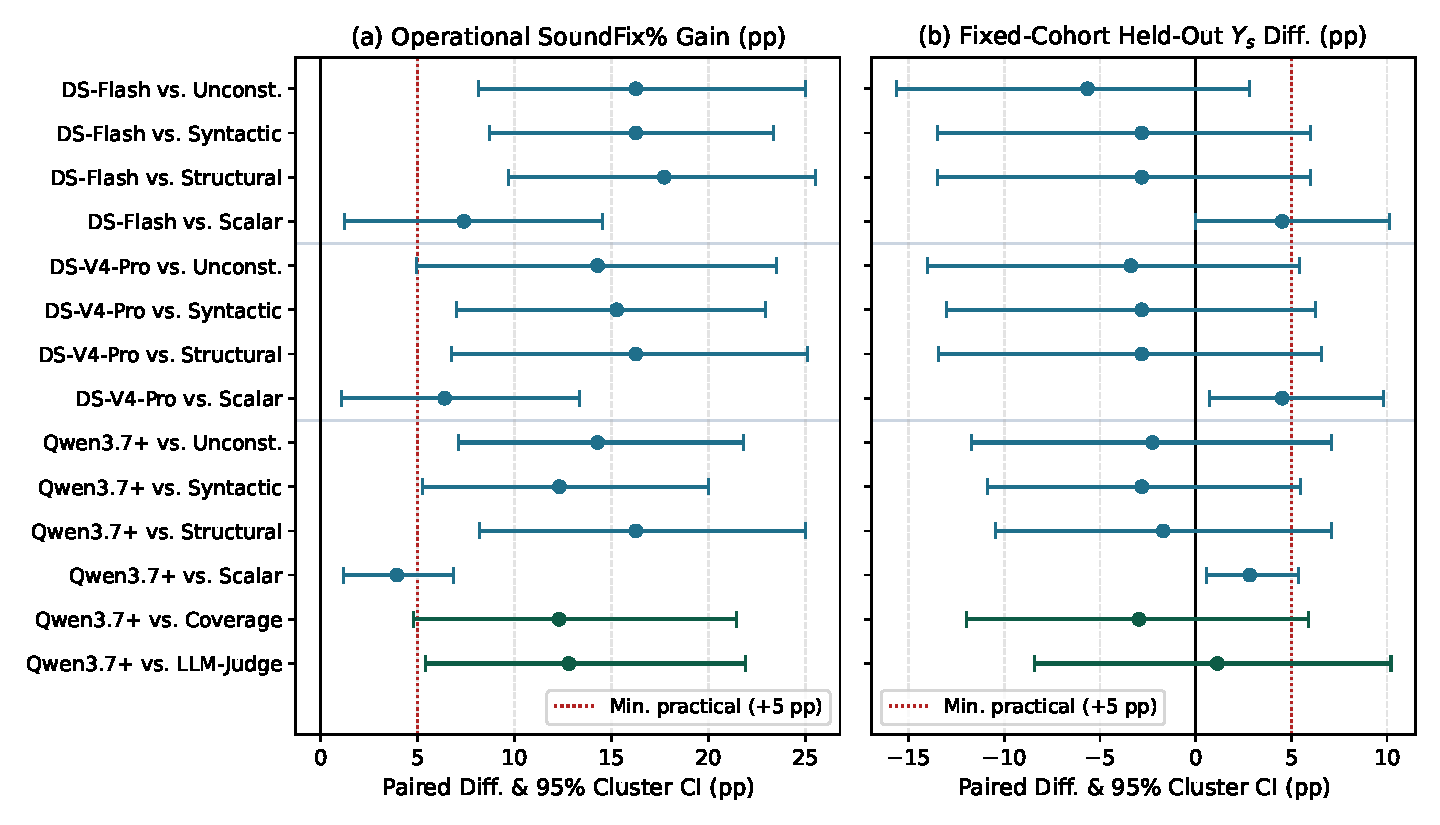
\includegraphics[width=0.96\textwidth]{figures/fig2_round_trajectories.pdf}
\caption{Whole-project clustered paired differences and 95\% confidence intervals for \textsc{MuGuard-Flake} on (a) operational sound-fix yield and (b) fixed-cohort held-out yield.}
\label{fig:forest_effects}
\end{figure*}

\paragraph{Causal Isolation of Surviving-Mutant Witnesses.}
The prefix-forked experiment across all $\ForkTotal$ frozen erosion states in $\ForkProjects$ repositories confirms that localized witnesses drive substantial recovery gains beyond gated retries alone (Table~\ref{tab:ablation} and Figure~\ref{fig:ablation_fork}). Supplying the True Witness package recovers \ForkAThreePct{} of eroded repairs, outperforming Scalar Ratio feedback (\ForkAOnePct{}) by 28.1 percentage points overall and by virtually the same margin under equal model weighting. This lift achieves clustered significance and holds across every model, spanning 20 points on confirmatory Qwen 3.7 Plus to 34 points on DeepSeek Flash.

Qualitative inspection of recovered trajectories explains why bare scalar ratios lag so sharply behind concrete witnesses. Told only that a few mutants survived, models often guess blindly, adding redundant assertions around the same weakened check or oscillating between two flaky variants. Given the exact surviving production line and source slice, by contrast, models immediately recognize the missed branch or truncated token and repair the root cause in a single follow-up turn.

\begin{table}[t]
\centering
\scriptsize
\setlength{\tabcolsep}{1.8pt}
\caption{Prefix-forked recovery from identical erosion states across all $\ForkTotal$ forks in $\ForkProjects$ repositories (100\% completed across all four arms).}
\label{tab:ablation}
\begin{tabular}{lrrrrr}
\toprule
Feedback Arm or Contrast & Mut. & Chars (Tok.) & Rec.\ / $n$ & Recovery\% [95\% CI] & Rds / $p$ ($p_{\text{Holm}}$) \\
\midrule
Gate-Only (Immediate Abstain) & 0.00 & 0 (0) & 0/129 & 0.00\% (def.) & --- \\
Scalar Ratio ($k/M$) & 0.00 & 530 (140) & 55/129 & 42.64\% [19.9, 70.3] & 1.25 \\
Misleading Witness (Stress) & 2.46 & 1901 (500) & 42/129 & 32.56\% [18.3, 52.7] & 1.50 \\
\textbf{True Witness (MuGuard)} & 2.46 & 1905 (501) & 91/129 & 70.54\% [53.4, 87.3] & 1.44 \\
\midrule
DS-Flash (True $-$ Scalar) & --- & --- & 33 vs.\ 18/44 & +34.09 [+9.09, +58.82] pp & 0.0625 \\
DS-V4-Pro (True $-$ Scalar) & --- & --- & 34 vs.\ 21/45 & +28.89 [+6.25, +52.83] pp & 0.0625 \\
Qwen3.7+ (True $-$ Scalar) & --- & --- & 24 vs.\ 16/40 & +20.00 [+8.70, +32.43] pp & 0.0312 \\
\midrule
\textbf{Pooled (True $-$ Scalar)} & --- & --- & 91 vs.\ 55/129 & \textbf{+27.91 [+11.70, +43.33] pp} & \textbf{0.0049 (0.0049)} \\
\textbf{Equal-Model (True $-$ Scalar)} & --- & --- & 3 models equal & \textbf{+27.66 [+11.80, +43.29] pp} & \textbf{0.0039} \\
\textbf{Pooled (True $-$ Misleading)} & --- & --- & 91 vs.\ 42/129 & \textbf{+37.98 [+24.32, +48.73] pp} & \textbf{0.0002 (0.0005)} \\
\bottomrule
\end{tabular}
\end{table}


The Misleading Witness arm confirms that diagnostic accuracy, not prompt verbosity, explains this gain. Keeping prompt structure and mutant count identical and pointing to already-killed mutants drops recovery to \ForkATwoPct{}, a 37.1-point deficit below True Witness on matched forks (Figure~\ref{fig:ablation_fork}). Models follow the misleading hint into irrelevant code regions, proving that mislocalized diagnostics actively harm recovery. Because roughly three-quarters of tests never trigger an erosion retry, that 28-point conditional lift translates into consistent full-cohort gains over Scalar Gate of 4 to 7 points in operational yield and 3 to 5 points in held-out yield (Figure~\ref{fig:forest_effects}). Gate enforcement and witness diagnostics thus play distinct, complementary roles: the gate stops silent erosion, and localized witnesses turn rejected drafts into valid fixes.

\begin{figure}[t]
\centering
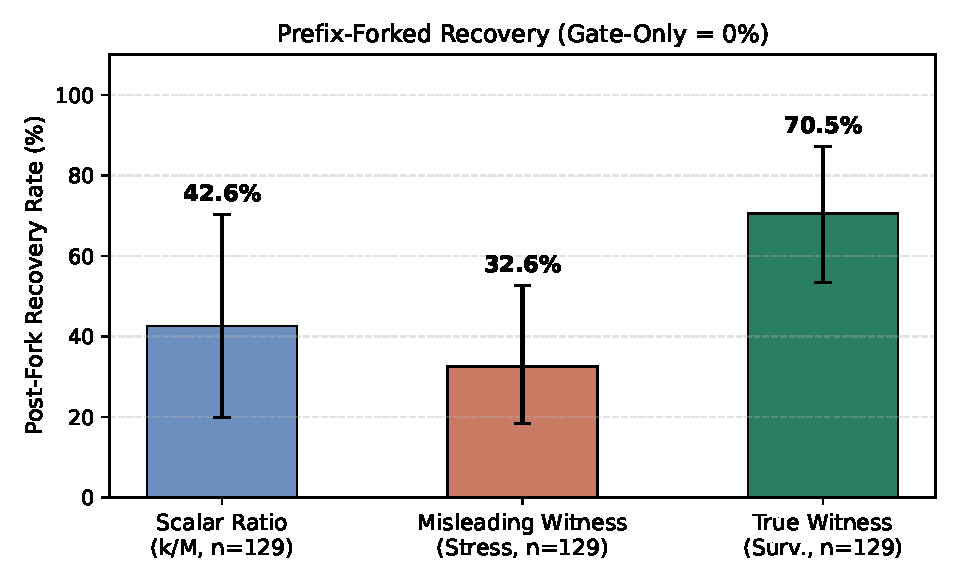
\includegraphics[width=0.74\textwidth]{figures/fig4_n14_ablation_and_pareto.pdf}
\caption{Post-fork recovery rates and 95\% cluster confidence intervals across feedback arms on frozen erosion states.}
\label{fig:ablation_fork}
\end{figure}

\medskip
\noindent\fbox{\parbox{0.97\textwidth}{\textbf{Summary for RQ3:} \textsc{MuGuard-Flake} eliminates in-loop erosion, raises operational sound-fix yield by 12 to 18 points over static guards, and cuts unseen held-out loss among accepted patches by 45\% to 65\%. Conservative abstention leaves unconditional held-out yield inconclusive, yet break-even analysis favors gating over non-mutation baselines whenever a silent regression costs more than 1.3 to 2.4 times an abstention review. Across $\ForkTotal$ prefix-forked states, localized witnesses outperform scalar feedback by 28 points.}}
\medskip

Having established the safety--coverage trade-off and witness mechanism in RQ3, RQ4 evaluates whether local mutation probing fits within practical CI latency budgets and what drives terminal abstentions.

\subsection{RQ4: Uncached Latencies, Abstentions, and Subset Sensitivity}
\label{sec:rq4}

\paragraph{Uncached Verification Latency vs.\ LLM Reasoning Cost.}
Local focal mutation probing is not the interactive bottleneck in automated flaky test repair (Table~\ref{tab:latency}). Even without caching, target mutation probing completes in a median of \LatUncachedJavaMutMed\,s on Java and \LatUncachedPyMutMed\,s on Python. Shared-scope partner probing adds 5.6\,s median in Java and 2.1\,s in Python.

Python's online gate runs more than three times faster than its single-run baseline sweep in Table~\ref{tab:benchmark} because the two stages probe different mutant sets. Offline baseline construction sweeps the full focal pool $M_{\text{focal}}$, including unkilled AST mutants and state-setter replays on OD-brittle tests. In-loop gating replays only the smaller frozen obligation subset $M_{\text{det}}$ (median 14 mutants) under standalone execution $e_{\text{iso}}$. In Java, PIT instruments covered focal classes as a unit on every invocation, keeping baseline and in-loop medians close.

By contrast, model inference dominates end-to-end repair time. Excluding network retry backoff, a single LLM reasoning call alone consumes a median of 53 to 80\,s across models. Including validation and retry rounds, end-to-end \textsc{MuGuard-Flake} sessions reach a median of 60\,s on DeepSeek Flash, 120\,s on DeepSeek V4 Pro, and 143\,s on Qwen 3.7 Plus. Within single-module CI builds, seconds-scale focal probing therefore adds only modest overhead on top of LLM generation, and short-circuiting compile or stability failures keeps probing focused strictly on viable candidates.

\begin{table}[t]
\centering
\scriptsize
\setlength{\tabcolsep}{4.0pt}
\caption{One-time $3\times$ baseline pre-computation times and uncached per-round validation stage latencies across Java and Python.}
\label{tab:latency}
\begin{tabular}{llrrrr}
\toprule
Phase & Stage / Scope & $n$ & Median (s) & IQR [P25, P75] (s) & P90 (s) \\
\midrule
Offline Pre-Comp.\ ($3\times M_{\text{focal}}$) & Java Default Mutators & 110 & 30.56 & [21.19, 42.44] & 60.30 \\
Offline Pre-Comp.\ ($3\times M_{\text{focal}}$) & Java Default+$M_{\text{ext}}$ & 110 & 39.39 & [22.39, 85.91] & 154.49 \\
Offline Pre-Comp.\ ($3\times M_{\text{focal}}$) & Python Baseline Pool & 93 & 37.10 & [23.46, 46.69] & 60.75 \\
\midrule
In-Loop Uncached (Java) & Compile & 960 & 4.07 & [2.47, 7.75] & 9.32 \\
In-Loop Uncached (Java) & Stability Reruns ($W^+$) & 891 & 4.21 & [1.95, 8.41] & 9.77 \\
In-Loop Uncached (Java) & Target Gate ($M_{\text{det}}$) & 716 & 9.51 & [6.16, 14.36] & 16.56 \\
In-Loop Uncached (Java) & Partner Gate ($M_{\text{det}}$) & 140 & 5.58 & [4.71, 5.90] & 6.34 \\
\midrule
In-Loop Uncached (Python) & Syntax Check & 219 & 0.01 & [0.01, 0.01] & 0.01 \\
In-Loop Uncached (Python) & Stability Reruns ($W^+$) & 669 & 1.00 & [0.95, 1.29] & 1.45 \\
In-Loop Uncached (Python) & Target Gate ($M_{\text{det}}$) & 495 & 3.72 & [2.64, 6.88] & 9.88 \\
In-Loop Uncached (Python) & Partner Gate ($M_{\text{det}}$) & 148 & 2.12 & [1.22, 2.98] & 4.57 \\
\bottomrule
\end{tabular}
\par\smallskip\parbox{0.96\textwidth}{\scriptsize\textit{Note:} Python in-loop gating replays only frozen killed obligations $M_{\text{det}}$ (median 14 mutants) under standalone $e_{\text{iso}}$, explaining its $3.3\times$ speedup relative to single-run full $M_{\text{focal}}$ baseline sweeps (12.29\,s in Table~\ref{tab:benchmark}; $3\times$ = 37.10\,s). Java PIT instruments covered classes per run, keeping baseline (10.21\,s) and in-loop (9.51\,s) medians close.}
\end{table}


\paragraph{Abstention Root Causes and Offline Subset Sensitivity.}
Unrecoverable oracle erosion accounts for only a minority of \textsc{MuGuard-Flake}'s terminal abstentions across the three multi-round models (25 on Flash, 28 on Pro, and 42 on Qwen). Across backbones, only five to nine tests end in erosion abstention, alongside two or three cases blocked by missing partner baseline coverage. Most abstentions stem instead from model formatting and stability limits, with malformed-patch sanity rejections and unstable reruns forming the bulk of terminal abstentions.

Inspecting those sanity rejections reveals a straightforward engineering root cause rather than an inherent flaw of mutation gating. In Python repositories, language models frequently emit class test methods with mismatched leading indentation, triggering immediate syntax rejection before stability or mutation checks even execute. Enforcing syntax-constrained decoding or deterministic method re-indentation would therefore recover substantial auto-merge coverage without weakening oracle protection.

Offline subset-sampling bounds across all \TaxUniquePatches{} unique eroded patches confirm two practical guidelines for gate configuration (Table~\ref{tab:topk} and Figure~\ref{fig:latency_topk}). First, omitting partner obligations caps maximum detection recall at 99.0\% even when probing all target mutants, because four eroded patches weaken exclusively partner obligations. Second, probing small subsets misses substantial erosion: uniform random sampling detects only 50.8\% of eroded patches at a 5-mutant budget and 68.9\% at 10 mutants, reaching 92.3\% at 25 mutants and outperforming line-dispersion and operator-priority heuristics at higher budgets.

\begin{table}[t]
\centering
\scriptsize
\setlength{\tabcolsep}{6.0pt}
\caption{Offline mutant subset-sampling detection recall across $\TaxUniquePatches$ unique eroded patches over joint target-and-partner obligation pools versus target-only probing.}
\label{tab:topk}
\begin{tabular}{lrrrrr}
\toprule
Sampling Budget & Pool Share & Uniform Random & File/Line Disp. & Operator Priority & Target-Only \\
\midrule
Top-1 & 5.1\% & 18.8\% & 19.5\% & 25.8\% & 20.7\% \\
Top-5 & 25.6\% & 50.8\% & 41.5\% & 42.8\% & 57.6\% \\
Top-10 & 44.6\% & 68.9\% & 64.2\% & 44.2\% & 75.5\% \\
Top-25 & 72.4\% & 92.3\% & 79.5\% & 84.0\% & 93.5\% \\
All & 100.0\% & 100.0\% & 100.0\% & 100.0\% & 99.0\% \\
\bottomrule
\end{tabular}
\par\smallskip\parbox{0.96\textwidth}{\scriptsize\textit{Note:} Target-Only omits partner obligations $M_{\text{det}}(T_{\text{part}})$, capping recall at 99.0\% because four eroded patches weaken exclusively partner obligations.}
\end{table}


That ordering reflects how behavioral erosion spreads across a repository. Heuristics that concentrate on a few lines or operator classes overlook faults in untouched helper methods, fixture branches, or partner classes, whereas uniform sampling covers the focal footprint more evenly. Even so, sampling trades away substantial safety for only a few seconds of saved compute. Because full single-test probing already completes in a median of under ten seconds, probing the complete target-and-partner obligation pool remains the clear default for CI merge gates.

\begin{figure*}[t]
\centering
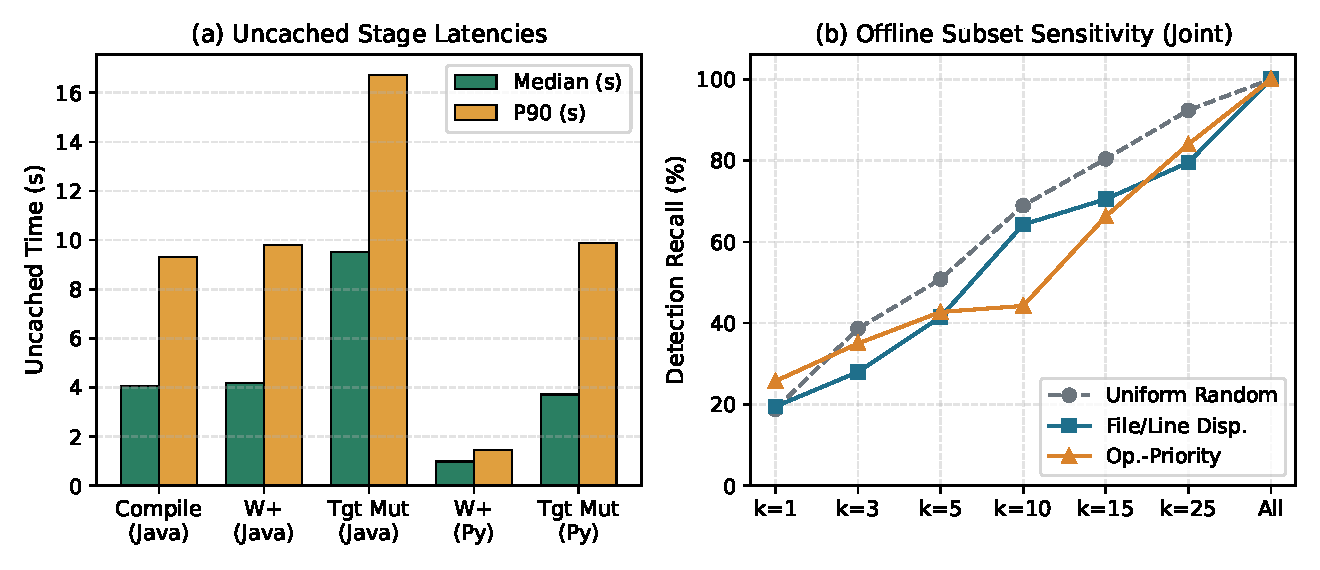
\includegraphics[width=0.95\textwidth]{figures/fig5_latency_distributions.pdf}
\caption{(a) Uncached in-loop stage latencies across Java and Python, and (b) offline subset-sampling detection recall over joint obligation pools.}
\label{fig:latency_topk}
\end{figure*}

\medskip
\noindent\fbox{\parbox{0.97\textwidth}{\textbf{Summary for RQ4:} Uncached in-loop probing takes under ten seconds median in Java and under four seconds in Python (replaying only frozen $M_{\text{det}}$ rather than full baseline $M_{\text{focal}}$), while LLM reasoning dominates session time. Most abstentions stem from Python formatting and stability limits rather than unrecoverable erosion, and full target-and-partner probing avoids both small-subset recall drops and partner-only blind spots.}}
\medskip
